% Options for packages loaded elsewhere
\PassOptionsToPackage{unicode}{hyperref}
\PassOptionsToPackage{hyphens}{url}
%
\documentclass[
]{article}
\usepackage{amsmath,amssymb}
\usepackage{lmodern}
\usepackage{iftex}
\ifPDFTeX
  \usepackage[T1]{fontenc}
  \usepackage[utf8]{inputenc}
  \usepackage{textcomp} % provide euro and other symbols
\else % if luatex or xetex
  \usepackage{unicode-math}
  \defaultfontfeatures{Scale=MatchLowercase}
  \defaultfontfeatures[\rmfamily]{Ligatures=TeX,Scale=1}
\fi
% Use upquote if available, for straight quotes in verbatim environments
\IfFileExists{upquote.sty}{\usepackage{upquote}}{}
\IfFileExists{microtype.sty}{% use microtype if available
  \usepackage[]{microtype}
  \UseMicrotypeSet[protrusion]{basicmath} % disable protrusion for tt fonts
}{}
\makeatletter
\@ifundefined{KOMAClassName}{% if non-KOMA class
  \IfFileExists{parskip.sty}{%
    \usepackage{parskip}
  }{% else
    \setlength{\parindent}{0pt}
    \setlength{\parskip}{6pt plus 2pt minus 1pt}}
}{% if KOMA class
  \KOMAoptions{parskip=half}}
\makeatother
\usepackage{xcolor}
\usepackage[margin=1in]{geometry}
\usepackage{graphicx}
\makeatletter
\def\maxwidth{\ifdim\Gin@nat@width>\linewidth\linewidth\else\Gin@nat@width\fi}
\def\maxheight{\ifdim\Gin@nat@height>\textheight\textheight\else\Gin@nat@height\fi}
\makeatother
% Scale images if necessary, so that they will not overflow the page
% margins by default, and it is still possible to overwrite the defaults
% using explicit options in \includegraphics[width, height, ...]{}
\setkeys{Gin}{width=\maxwidth,height=\maxheight,keepaspectratio}
% Set default figure placement to htbp
\makeatletter
\def\fps@figure{htbp}
\makeatother
\setlength{\emergencystretch}{3em} % prevent overfull lines
\providecommand{\tightlist}{%
  \setlength{\itemsep}{0pt}\setlength{\parskip}{0pt}}
\setcounter{secnumdepth}{-\maxdimen} % remove section numbering
\ifLuaTeX
  \usepackage{selnolig}  % disable illegal ligatures
\fi
\IfFileExists{bookmark.sty}{\usepackage{bookmark}}{\usepackage{hyperref}}
\IfFileExists{xurl.sty}{\usepackage{xurl}}{} % add URL line breaks if available
\urlstyle{same} % disable monospaced font for URLs
\hypersetup{
  hidelinks,
  pdfcreator={LaTeX via pandoc}}

\author{}
\date{\vspace{-2.5em}}

\begin{document}

\hypertarget{surds}{%
\section{Surds}\label{surds}}

\hypertarget{notes-and-examples}{%
\subsection{Notes and examples}\label{notes-and-examples}}

\hypertarget{rational-and-irrational-numbers}{%
\subsubsection{Rational and irrational
numbers}\label{rational-and-irrational-numbers}}

An irrational number is a number which cannot be expressed as one whole
number divided by another whole number. Irrational numbers can't be
written as fractions.

The square root of any number which is not itself a perfect square is an
irrational number. So \(\sqrt{2}\) and \(\sqrt{3}\) are irrational
numbers, but \(\sqrt{4}\) is not as it is equal to 2, which is a
rational number. A number which is partly rational and partly square
root (or cube root etc.) is called a surd. (There are of course other
irrational numbers which do not involve a root, such as \(\pi\)

In this section you will learn to manipulate and simplify expressions
involving surds. This is an important skill in many areas of
mathematics. For example, suppose you have a triangular paving slab like
this:

\begin{figure}
\centering
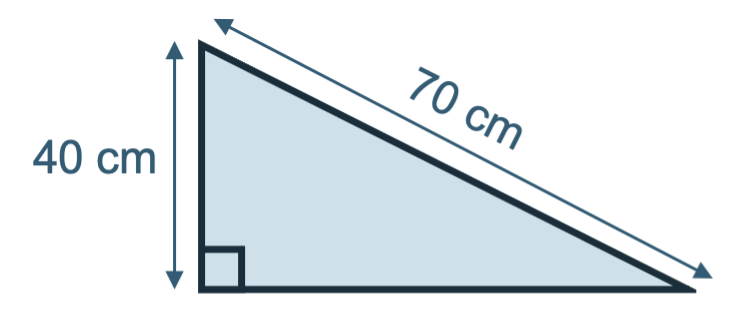
\includegraphics[width=2.60417in,height=\textheight]{images/Picture.png}
\caption{right angled triangle with hypotenuse 70cm and a shorter side
of 40cm}
\end{figure}

You can use Pythagoras' theorem to work out that the length of the third
side is \(\sqrt{3000}\). You could use a calculator to work this out and
give the answer to two or three decimal places, but this would no longer
be exact. Suppose you wanted to find the area and perimeter of the slab,
or the total area of 100 slabs, or find out how many slabs you could
make from a certain volume of concrete? It is much better to use the
exact answer in these calculations, and then the results will also be
exact.

\hypertarget{writing-a-square-root-in-terms-of-a-simpler-square-root}{%
\subsubsection{Writing a square root in terms of a simpler square
root}\label{writing-a-square-root-in-terms-of-a-simpler-square-root}}

Square roots like the one in the example above look quite daunting and
can be difficult to work with. However, many square roots can be written
in terms of a simpler square root like \(\sqrt{2}\) or \(\sqrt{3}\) (and
the same applies to cube roots and so on). Example 1 shows how to do
this.

\textbf{Example 1}

Write these numbers in terms of the simplest possible square roots.

\begin{enumerate}
\def\labelenumi{(\alph{enumi})}
\tightlist
\item
  \(\sqrt{12}\)\\
\item
  \(\sqrt{72}\)\\
\item
  \(\sqrt{150}\)
\end{enumerate}

\textbf{\emph{Solution}}

\begin{enumerate}
\def\labelenumi{(\alph{enumi})}
\item
  \(\begin{aligned} &12=4\times 3 \\ &\sqrt{12}=\sqrt{4} \times \sqrt{3}=2\sqrt{3} \\ \end{aligned}\)
\item
  \(\begin{aligned} &72=36\times 2 \\ &\sqrt{72}=\sqrt{36} \times \sqrt{2}=6\sqrt{3} \\ \end{aligned}\)
\item
  \(\begin{aligned} &150=25\times 6 \\ &\sqrt{150}=\sqrt{25} \times \sqrt{6}=5\sqrt{6} \\ \end{aligned}\)
\end{enumerate}

\hypertarget{adding-and-subtracting-surds}{%
\subsubsection{Adding and subtracting
surds}\label{adding-and-subtracting-surds}}

Adding and subtracting surds is rather like adding or subtracting
algebraic expressions, in that you have to collect ``like terms''. You
should collect together any rational numbers, and collect together any
terms involving roots of the same number. You cannot collect together
terms involving roots of different numbers, such as \(\sqrt{2}\) and
\(\sqrt{3}\).

\textbf{Example 2}

Simplify

\begin{enumerate}
\def\labelenumi{(\alph{enumi})}
\tightlist
\item
  \((2+\sqrt{2})+(3-2\sqrt{2})\)
\item
  \((4-\sqrt{3})-(1-2\sqrt{2}+3\sqrt{3})\)
\item
  \(\sqrt32-\sqrt{18}\)
\end{enumerate}

\textbf{\emph{Solution}}

\begin{enumerate}
\def\labelenumi{(\alph{enumi})}
\item
  \(\begin{aligned} (2+\sqrt{2})+(3-2\sqrt{2}) &= 2+3+\sqrt{2}-2\sqrt{2} \\ &=5-\sqrt{2} \end{aligned}\)
\item
  \(\begin{aligned} (4-\sqrt{3})-(1-2\sqrt{2}+3\sqrt{3}) &= 4-\sqrt{3}-1+2\sqrt{2}-3\sqrt{3} \\ &=4-1-\sqrt{3}-3\sqrt{3}+2\sqrt{2} \\ &=3-4\sqrt{3}+2\sqrt{2} \end{aligned}\)
\item
  \(\begin{aligned} &\textit{At first sight this looks like it cannot be simplified. However, both surds can be written in terms of simpler surds (as in Example 1).} \\ &\sqrt{32}=\sqrt{16}\times\sqrt{2}=4\sqrt{2} \\ &\sqrt{18}=\sqrt{9}\times\sqrt{2}=3\sqrt{2} \\ &\sqrt{32}-\sqrt{18}=4\sqrt{2}-3\sqrt{2}=\sqrt{2} \\ \end{aligned}\)
\end{enumerate}

\hypertarget{multiplying-surds}{%
\subsubsection{Multiplying surds}\label{multiplying-surds}}

Multiplying two or more square roots is quite simple -- you just
multiply the numbers. You may then be able to write the result as a
simpler surd.

\textbf{Example 3}

Simplify

\begin{enumerate}
\def\labelenumi{(\alph{enumi})}
\item
  \(\sqrt 2 \times \sqrt 6\)
\item
  \(2\sqrt {15} \times \sqrt 6 \times 3\sqrt {10}\)
\end{enumerate}

\textbf{\emph{Solution}}

\begin{enumerate}
\def\labelenumi{(\alph{enumi})}
\tightlist
\item
  \(\begin{array}{l} \sqrt 2 \times \sqrt 6 &= \sqrt {12} \\  &= \sqrt 4 \times \sqrt 3 \\  &= 2\sqrt 3 \end{array}\)
\end{enumerate}

\emph{The approach used in part (a) works well for small numbers, but
for part (b) you would get the square root of a large number to
simplify. An easier way for this example is to split each surd into
simpler ones and then look for any pairs.}

\begin{enumerate}
\def\labelenumi{(\alph{enumi})}
\setcounter{enumi}{1}
\tightlist
\item
  \(\begin{array}{l} 2\sqrt {15} \times \sqrt 6 \times 3\sqrt {10} &= (2 \times \sqrt 3 \times \sqrt 5 ) \times (\sqrt 2 \times \sqrt 3 ) \times (3 \times \sqrt 5 \times \sqrt 2 )\\  &= 2 \times 3 \times \sqrt 3 \times \sqrt 3 \times \sqrt 5 \times \sqrt 5 \times \sqrt 2 \times \sqrt 2 \\  &= 6 \times 3 \times 5 \times 2\\  &= 180 \end{array}\)
\end{enumerate}

The next example deals with multiplying expressions involving a mixture
of rational numbers and roots. You have to use brackets for this, and it
is very similar to multiplying out two brackets in algebra -- each term
in the first bracket needs to be multiplied by each term in the second
bracket. You can use FOIL (First, Outer, Inner, Last) if it helps you.

\textbf{Example 4}

Multiply out and simplify

\begin{enumerate}
\def\labelenumi{(\alph{enumi})}
\tightlist
\item
  \((2 + \sqrt 3 )(1 - 2\sqrt 3 )\)
\item
  \({(3 - \sqrt 2 )^2}\)
\item
  \((\sqrt 5 - 2)(\sqrt 5 + 2)\)
\end{enumerate}

\textbf{\emph{Solution}}

\begin{enumerate}
\def\labelenumi{(\alph{enumi})}
\item
  \(\begin{align} (2 + \sqrt 3 )(1 - 2\sqrt 3 ) &= 2 - 4\sqrt 3 + \sqrt 3 - 2\sqrt 3 \times \sqrt 3 \\  &= 2 - 3\sqrt 3 - 6\\  &= - 4 - 3\sqrt 3 \end{align}\)
\item
  \(\begin{align} {(3 - \sqrt 2 )^2} &= (3 - \sqrt 2 )(3 - \sqrt 2 )\\  &= 9 - 3\sqrt 2 - 3\sqrt 2 + \sqrt 2 \times \sqrt 2 \\  &= 9 - 6\sqrt 2 + 2\\  &= 11 - 6\sqrt 2 \end{align}\)
\item
  \(\begin{align} (\sqrt 5 - 2)(\sqrt 5 + 2) &= \sqrt 5 \times \sqrt 5 + 2\sqrt 5 - 2\sqrt 5 - 2 \times 2\\  &= 5 - 4\\  &= 1 \end{align}\)
\end{enumerate}

Part (c) of Example 4 illustrates a very important and useful idea.
Multiplying out any expression of the form \((a+b)(a-b)\) gives the
result \(a^{2}-b^{2}\). The ``outer'' and ``inner'' products,\(-ab\) and
\(ab\), cancel each other out. When either or both of \emph{a} and
\emph{b} are surds, the result \(a^{2}-b^{2}\) is a rational number.

\hypertarget{rationalising-the-denominator}{%
\subsubsection{Rationalising the
denominator}\label{rationalising-the-denominator}}

Surds in the denominator of a fraction can be a real nuisance! However,
you can get rid of them from the denominator by a process called
rationalising the denominator, which uses the idea above. If the
denominator of a fraction is \emph{a} + \emph{b}, where either or both
of \emph{a} and \emph{b} are surds, then you can multiply both top and
bottom of the fraction by \emph{a} -- \emph{b}. The denominator is then
\((a+b)(a-b)\), which expands to give a rational number. Since you
multiply the top and bottom of the fraction by the same amount, its
value is unchanged. The numerator still involves surds, but this is not
quite so difficult to work with.

This technique is shown in Example 5.

\textbf{Example 5}

Simplify the following by rationalising the denominator.

\begin{enumerate}
\def\labelenumi{(\alph{enumi})}
\item
  \(\frac{1}{{\sqrt 3 }}\)
\item
  \(\frac{1}{{\sqrt 2 + 1}}\)
\item
  \(\frac{{2 + \sqrt 3 }}{{1 - \sqrt 3 }}\)
\end{enumerate}

\textbf{\emph{Solution}}

\emph{Remember if the denominator of a fraction is a surd then the
fraction is not in its simplest form.}

\(\begin{align} \textbf{a.} \hspace{1em} \frac{1}{{\sqrt 3 }} &= \frac{1}{{\sqrt 3 }} \times \frac{{\sqrt 3 }}{{\sqrt 3 }}\\  &= \frac{{\sqrt 3 }}{3} \end{align}\)

\(\begin{align} \textbf{b.} \hspace{1em} \frac{1}{{\sqrt 2 + 1}} &= \frac{1}{{\sqrt 2 + 1}} \times \frac{{\sqrt 2 - 1}}{{\sqrt 2 - 1}}\\  &= \frac{{\sqrt 2 - 1}}{{(\sqrt 2 + 1)(\sqrt 2 - 1)}}\\  &= \frac{{\sqrt 2 - 1}}{{2 - 1}}\\  &= \sqrt 2 - 1 \end{align}\)

\(\begin{align} \textbf{c.} \hspace{1em} \frac{{2 + \sqrt 3 }}{{1 - \sqrt 3 }} &= \frac{{2 + \sqrt 3 }}{{1 - \sqrt 3 }} \times \frac{{1 + \sqrt 3 }}{{1 + \sqrt 3 }}\\  &= \frac{{(2 + \sqrt 3 )(1 + \sqrt 3 )}}{{(1 - \sqrt 3 )(1 + \sqrt 3 )}}\\  &= \frac{{2 + 2\sqrt 3 + \sqrt 3 + 3}}{{1 - 3}}\\  &= - {\textstyle{1 \over 2}}(5 + 3\sqrt 3 ) \end{align}\)

\end{document}
